\chapter{\IfLanguageName{dutch}{Literatuurstudie}{State of the art}}
\label{ch:literatuurstudie}

Dit hoofdstuk zal een overzicht geven van de theoretische achtergrond van de hardware, protocollen, programma's en andere concepten die gebruikt zullen worden bij het gevoerde onderzoek voor het beantwoorden van bovengenoemde onderzoeksvraag.

\section{Definities}
Deze sectie zal enkele belangrijke begrippen introduceren die belangrijk zullen zijn bij het verdere lezen van dit hoofdstuk en de rest van het document.

\subsubsection{RSSI}
De RSSI, of voluit Received Signal Strength Indicator, is een maat voor de signaalsterkte die een ontvanger ontvangt van bijhorende zender. Ze wordt typisch gebruikt als het over radio-/elektromagnetische golven gaat.\autocite{Admin2022} Ze wordt uitgedrukt in Dbm (Decibel per milliwatt).\autocite{Tseard2016} Het is een zeer kleine en logaritmische maat, de waarden in dit document zullen in de grootteorde -10 Dbm liggen.

\subsubsection{IoT}
IoT, of voluit Internet Of Things, is een systeem van samenwerkende devices die met elkaar verbonden zijn via het internet, en zo, zonder menselijke tussenkomst, taken uitvoeren. Elk device is geïdentificeerd door een unieke identifier, of UID. Een device in deze context is alles wat met het internet kan verbonden zijn.\autocite{Gillis2022}

\subsubsection{MQTT}
MQTT, of voluit Message Queuing Telemetry Transport, is een protocol voor het versturen van berichten gemaakt door IoT devices over het internet. Belangrijke voordelen van het protocol zijn dat het licht en efficiënt is, en gemakkelijk schaalbaar naar grote hoeveelheden devices.\autocite{MQTT2022}

\subsubsection{FSPL}
FSPL, of voluit Free Space Path Loss, is het theoretische verlies in signaalsterkte over een bepaalde afstand in open ruimte. Deze kan berekend worden, gegeven de afstand tussen de 2 antennes (d), de frequentie van de EM golf (f), en de gain op de zendende en ontvangende antenne (Gz en Go respectievelijk). Ze wordt berekend via onderstaande formule: 
\[FSPL = 20\log_{10}(d) + 20\log_{10}(f) + 20\log_{10}(\frac{4\pi}{c}) - G_z - G_o \]
\autocite{Pasternack2020}

\subsubsection{Trilateratie}
Trilateratie is de berekening voor de bepaling van de coördinaten van een punt uit 2 geweten punten, en de afstanden van die punten tot het te berekenen punt. Hierbij blijft ook een zogenaamd 'dubbelzinnig punt' over, welk logisch moet worden uitgebrand. De formules voor berekening zijn als volgt:
 \[x = \frac{d_1^2 - d_2^2 + (x_2 - x_1)}{2(x_2 - x_1)} + x_1\]
 \[y = \sqrt{d_1^2 - x^2} \pm y_1\]
 Met \((x,  y)\) de coördinaten van het onbekende punt,  \((x_1, y_1)\) en \((x_2, y_1)\) de coördinaten van de geweten punten en \(d_1\) en \(d_2\) de bekende afstanden.
 \autocite{TRM2022}

\section{Hardware}
\label{sec:Hardware}
Deze sectie zal de gebruikte hardwaretechnologieën toelichten, deze zijn RFID en BLE.

\subsection{RFID}
\label{sec:RFID}
RFID, of voluit Radio Frequency IDentification, is een draadloos communicatie systeem welke gebruik maakt van elektromagnetische golven. Een typische RFID opstelling bestaat uit 3 delen, nl. een zender/ontvanger combinatie of transceiver, een antenne, en een transponder of RFID-tag.\autocite{Auxcis2022} In essentie werkt dit als volgt: de transmitter laat de antenne een elektromagnetisch veld opwekken. Alle RFID-tags die zich in dit veld bevind zullen dit registreren en zij zullen ook een veld opwekken, welke op zijn beurt dan terug zal opgevangen worden door de antenne, waarna dit zal doorgegeven worden aan de receiver.. 
% TODO: afbeelding refereren
\begin{figure}[h]
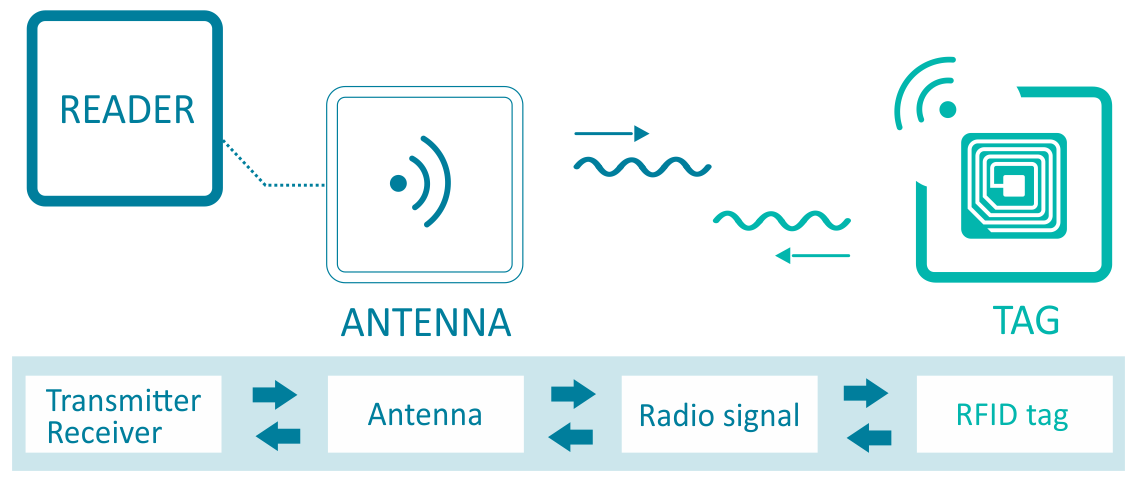
\includegraphics{werking_rfid}
\centering
\end{figure}
In essentie zal de transmitter dus een signaal uitsturen, waarop alle RFID-tags binnen bereik zullen antwoorden, waarna dit antwoord terug zal belanden bij de receiver. De combinatie van de transceiver en de antenne wordt vaak een RFID lezer of reader genoemd, aangezien deze onderdelen steeds samen moeten werken en hardwarematig op 1 locatie zullen staan.\autocite{Amster2021}
Deze transceiver is echter meestal niet gelimiteerd tot slechts 1 aangesloten antenne, afhankelijk van de gebruikte hardware kan deze ook 2 of 4 antennes aankoppelen. De data die de transceiver ontvangt van de RFID-tags kan vervolgens via diverse kanalen verzonden worden naar een computer of server die deze dan verder kan afhandelen.

Alhoewel alle onderdelen in de opstelling in vele verschillende geuren en kleuren beschikbaar zijn, verschilt de functionaliteit bij de antenne en transceiver niet zozeer. De antennes kunnen verschillen in oppervlakte en vorm. Dit heeft invloed op de zone waaruit RFID-tags antwoorden zullen sturen. Een vlakke antenne stuurt voor zich uit, dus verwacht antwoorden van uit die richting, terwijl een staafvormige rondom zich straalt maar niet naar zijn uiteinden. De vorm van antenne beïnvloed ook de polarisatie van het EM veld, welke ook een invloed heeft op de RSSI. De keuze keuze tussen deze verschillende mogelijkheden is dus duidelijk afhankelijk van het toepassingsgebied. Ook de zendstekte kan variëren, maar deze is instelbaar (binnen grenzen bepaald door de transmitter). Echter blijft het hier qua verschillen voornamelijk bij. De RFID-tag daarentegen heeft veel meer fundamentele verschillen en types, welke ook een uitgebreide uitleg nodig hebben wil de lezer het komende onderzoek kunnen volgen.

\subsubsection{De RFID-tag}
\label{sec:De RFID-tag}
Een RFID-tag, in zijn eenvoudigste vorm, bestaat uit 2 delen, nl. een IC of computerchip, en een antenne. Deze vorm wordt een passieve RFID-tag genoemd. Sommige tags beschikken ook over een interne batterij, deze actieve RFID-tags worden echter niet gebruikt tijdens dit onderzoek, en worden dus verder buiten beschouwing gelaten.\autocite{atlasrfidstore2022} 

De IC in de antenne is het brein van de chip. Natuurlijk heeft hij, door zijn kleine gestalte, niet veel functionaliteit. De chip bevat 4 memory banks (slots voor data), van variabele lengte (verschillende producenten produceren chips met verschillende groottes per dataslot). Deze slots zijn als volgt: de EPC (Electronic Product Code), welke een code bevat die geplaatst is door de producent maar veranderbaar is door de gebruiker. De TID (Tag Identifier), welke een uniek, read-only tagnummer bevat. De User memory, waar de gebruiker data kan opslaan, en de Reserved Memory bank, welke beveiligingsdata bevat voor het veranderen van de user memory.\autocite{Smiley2017} Deze laatste 2 zullen ongebruikt blijven bij dit onderzoek aangezien de data in de chip niet belangrijk is, maar vooral de locatie en de identificatie van de chip.

Het 2e deel van de tag, de antenne, beslaat fysiek de grootste oppervlakte van de tag. De taak van dit onderdeel is de EM signalen, uitgezonden door de transmitter, op te vangen. Waarna dit signaal gemoduleerd wordt in functie van de opgeslagen data in de dataslots en ze daarna teruggezonden wordt. Aangezien deze tags niet over een interne batterij beschikken, kaatsen ze de energie van de transmitter terug (in een licht andere golflengte en ritme door het moduleren). Dit wordt backscattering genoemd. Door deze relatie is de signaalsterkte van de transmitter dus even verantwoordelijk voor de RSSI, als de afstand tussen de tag en de antenne. Daarom is dit ook een zeer belangrijke variabele in dit verdere onderzoek.\autocite{atlasrfidstore2022a}

\subsubsection{RSSI beïnvloedende factoren}
\label{sec:RSSI beïnvloedende factoren}
In de voorgaande paragrafen zijn al enkele factoren opgesomd die de RSSI beïnvloeden, echter zijn dit niet de enige. Zo hebben we de zogenaamde SOAP: Size, Orientation, Angle en Placement.
\begin{itemize}
	\item \underline{Size}:
	De grootte van een tag, of specifieker van de antenne, is zeer belangrijk voor de RSSI die de receiver terug ontvangt. Hoe groter het antenneoppervlak, hoe meer energie van de originele golf wordt opgenomen, en hoe sterker het teruggezonden signaal zal zijn.
	\item \underline{Orientation en Angle}:
	Deze 2 hangen grotendeels samen. Over het algemeen zal de opgenomen energie door de antenne, en dus de RSSI van de terugzending, het hoogst zijn als het EM veld recht op de antenne staat. Hoe meer van deze staat afgeweken wordt hoe minder de RSSI dus zal zijn. Het verdraaien van de tag zal dus een grote invloed hebben op de RSSI. 
	\item \underline{Placement}:
	Waar de tag (op) geplaatst wordt heeft ook een grote invloed. Allereerst is heeft alles wat tussen de tag en de reader wordt geplaatst heeft een negatieve invloed op de RSSI, dit kan gaan van stof (bv. een RFID toegangskaart in een broekzak) welke een verwaarloosbare invloed heeft, tot een ijzeren plaat, welke zo'n grote invloed heeft dat er quasi geen signaal meer zal zijn. Dit is dus een belangrijke beschouwing naargelang de use case. Verder is het zo dat RFID-tags die op een metalen oppervlakte of een waterhoudende container (water heeft ook een grote invloed) worden geplaatst (ook al hangen ze richting de antenne) een speciale isolerende plaklaag moeten hebben om interferentie te voorkomen.
\end{itemize}

Buiten deze voorgaande factoren zijn er nog enkele factoren die minder te beïnvloeden zijn, zoals tussenliggende kabels en andere hardware (zoals een multiplexer) tussen de antenne en de receiver. Elk onderdeel waar het signaal door moet heeft een invloed op de RSSI, ook al is deze meestal verwaarloosbaar klein.\autocite{Armstrong2013}

De oplettende lezer heeft al opgemerkt dat deze factoren een grote invloed kunnen hebben op de resultaten van dit onderzoek. Uiteraard zullen alle testen moeten gebeuren in een gecontroleerde omgeving, waar de invloed van deze factoren zo veel mogelijk zal worden geminimaliseerd. De specifieke uitwerking hieromtrent is vindbaar onder Hoofdstuk~\ref{ch:methodologie}.

\subsection{BLE}
\label{sec:BLE}
BLE, of voluit Bluetooth Low Energy, is een opvolger van de klassieke Bluetooth (meer specifiek is het versie 4.0). Het is zoals zijn voorganger dus ook een standaard voor korte afstand datatransfer. Waarin het echter verschilt is dat het minder energie verbruikt, vandaar het low energy gedeelte van de naam. Het bereikt dit door lagere transfer snelheden, en het feit dat het data verzend in korte packets, en tussen de zendingen in slaapstand gaat. Dit in tegenstelling tot klassieke Bluetooth, welke een blijvende connectie onderhoud en dus nooit slaapt. Dit betekend dat BLE tot wel 100x minder energie kan verbruiken dan klassieke Bluetooth. \autocite{Nesbo2021}

In de context van dit onderzoek zal deze vorm van datatransfer gebruikt worden in een set-up die bestaat uit 2 delen (waarvan er van elk 1 of meerdere aanwezig zijn), nl. BLE beacons en IoT gateways.

\subsubsection{De BLE beacon}
BLE beacons zijn de devices die het feitelijke BLE signaal zullen versturen. Dit zijn actieve sensors, wat inhoud dat ze beschikken over een interne batterij en dat ze, ongeacht wie of wat er luistert, berichten versturen, en dit met een bepaald tijdsinterval. Deze intervallen zijn vrij kort en worden normaal uitgedrukt in ms.\autocite{Adarsh2022}
De berichten die verstuurd worden bevatten het UID van de beacon, alsook mogelijk diverse andere informatie. De informatie die verzonden wordt hangt echter af van het protocol welke gebruikt wordt. Momenteel zijn de 3 voornaamste protocollen op de markt de volgende:
\begin{itemize}
	\item \underline{IBeacon}:
	Chronologisch het eerst uitgekomen BLE hardware en transferprotocol. Uitgebracht door Apple in 2013. 
	\item \underline{AltBeacon}:
	Een open-source tegenhanger voor het IBeacon platform van Apple, uitgebracht in 2014.
	\item \underline{Eddystone}:
	Het antwoord van Google op de BLE protocol markt, uitgebracht in 2015. Dit is het protocol welke zal gebruikt worden tijdens dit onderzoek en zal verder in detail worden uiteengezet.
\end{itemize}
Hoewel deze protocols zijn uitgebracht door verschillende (rivaliserende) bedrijven, zijn ze allen beschikbaar voor zowel Android als IOS.\autocite{Smart2022}

Het aanbod beacons op de markt is vrij uitgebreid, en de meeste zijn ook samen bruikbaar in een systeem mits ze zijn ingesteld met hetzelfde protocol. Tegenwoordig beginnen sommige fabrikanten echter eigen protocollen uit te werken, welke in sommige situaties eventueel beter zouden werken maar deze laten we hier buiten beschouwing aangezien dit risico's brengt naar uitbreiding van systemen toe. In dit onderzoek kiezen we voor een standaard protocol.

Aangezien deze beacons een batterij bevatten, is batterijduur ook een belangrijk aandachtspunt aangezien deze een rechtstreekse invloed heeft op de onderhoudskost van systemen die vertrouwen op deze beacons. Deze duur wordt voornamelijk beinvloed door de zendfrequentie en de grootte van de gestuurde berichten, ook kan het een optie zijn een tag met een grotere batterij te gebruiken, maar deze zijn groter en duurder. Qua performance heeft dit geen invloed maar wel op de kostprijs. 

\subsubsection{Een IoT Gateway}
Zoals de naam doet vermoeden is deze gateway niet specifiek voor BLE, maar is het een intelligente hub voor IoT toepassingen algemeen, het is een device dat IoT devices kan verbinden met het internet en is in een IoT systeem dus onmisbaar. Een BLE beacon is echter ook een IoT device dus dit is een perfecte toepassing voor zo'n Gateway.\autocite{MultiTech2022} Een Gateway kan ook filteren en enige datamanipulatie doen, dit is nodig aangezien niet enkel de BLE beacons een signaal verzenden, maar zowat elk modern draadloos device dit doet. Zonder filtering zijn door het bos de bomen niet meer zichtbaar. Parallel aan dit feit wilt dit ook zeggen dat de meeste hedendaagse devices, zoals smartphones, tablets en pc's gebruikt kunnen worden als gateway of om BLE signalen op te vangen, door middel van een programma zoals nRF Connect.\autocite{Semiconductor2022}.

\subsubsection{Het Eddystone protocol}
Zoals eerder vermeld is Eddystone het protocol welke gebruikt zal worden voor deze testen, en wordt hier verder in detail besproken. Eddystone is een BLE protocol ontworpen door Google en wordt onderhouden sinds 2015. Het bestaat uit berichten met 3 verschillende frame types. 
% TODO: afbeelding refereren
\begin{figure}[h]
	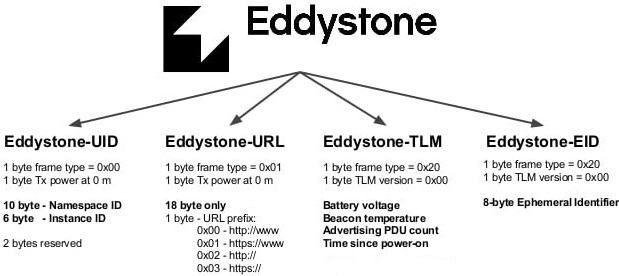
\includegraphics{eddystone_formats}
	\centering
\end{figure}
\begin{itemize}
	\item \underline{UID}:
	Dit frame (frametype x00) is het frame voor de broadcasting van het unieke beacon ID, of UID. Het bevat ook een veld genaamd 'Tx Power at 0m', dit is bedoeld om de RSSI waarde op 0m van de beacon mee te geven. Dit kan voor sommige toepassingen belangrijk zijn aangezien de standaard RSSI verschilt tussen verschillende beacon types, en er ook de mogelijkheid bestaat om een offset aan deze RSSI in te stellen.
	\item \underline{URL}:
	Dit frame (frametype x10) is bedoeld voor de broadcasting van een URL. Bij de ontwikkeling was het de bedoeling om notificaties met advertenties te laten zien op smartphones bij het voorbij wandelen van een BLE beacon via een bestemmings-URL verzonden via dit frame. Dit is echter nooit commercieel aangeslagen en Google ondersteund deze functie niet meer sinds december 2018.\autocite{Estimote2018} Deze frames zijn echter niet geheel nutteloos aangezien de verzonden URL ingesteld kan worden en dus kan gebruikt worden om custom data door te sturen.
	\item \underline{TLM}:
	TLM is kort voor Telemetry, dit frame (frametype x20) wordt gebruikt voor het verzenden van data over de beacon. Meer bepaald over de stand van de batterij, de temperatuur van de beacon, en het aantal verzonden berichten en verstreken tijd sinds het in gebruik nemen. Eddystone is het enige protocol dat dit doet en dit is een van de voordelen van dit protocol. Het frametype x20 wordt ook nog voor andere berichten gebruikt die niet in het oorspronkelijke protocol zaten, zoals EID (Ephemeral IDentifier), welke gebruikt wordt voor beveiliging en encryptie.
\end{itemize}\autocite{Google2018}

\section{Software}
\label{sec:Software}
Deze sectie zal de voornaamste software die gebruikt zal worden tijdens het onderzoek toelichten.

\subsubsection{ARTA}
ARTA, of voluit Aucxis RFID Testing Application, is het custom testprogramma van Aucxis. Deze zal gebruikt worden voor het testen van de RFID opstellingen, en het visualiseren van de data.

\subsubsection{RabbitMQ}
RabbitMQ is een Open source message broker. Het is een programma welke berichten binnenkrijgt, deze in een lijst steekt, en deze doorstuurt naar een ontvanger. Hoe, naar waar en de transformaties op de berichten zijn instelbaar. In praktijk zal dit gebruikt worden bij de BLE opstellingen om de BLE berichten van die verkregen worden door de IoT gateway gebundeld door te sturen naar een bepaald adres op het web via het MQTT protocol, waar deze dan zichtbaar zijn voor onderzoek.\autocite{RabbitMQ2022}

\subsubsection{MQTT Explorer}
MQTT Explorer is een programma voor het accepteren en visualiseren van berichten verstuurd over MQTT, deze zal gebruikt worden om de berichten verstuurd door RabbitMQ op te vangen zodat ze zichtbaar zijn voor visualisatie.\autocite{Nordquist2019}

\subsubsection{Hertz}
Hertz is het custom middleware platform van Aucxis. Deze zorgt voor de verbinding tussen ofwel MQTT berichten bij BLE en de lezer bij RFID eenderzijds, en een API anderzijds. Deze zal gebruikt worden als de verkregen data geanaliseerd moet worden via een script of dergelijke en op een computer moet geraken.\autocite{Hertz2020}